\documentclass[11pt]{beamer}
\usetheme{Boadilla}
\usecolortheme{seahorse}
\usepackage{tikz}
\usepackage{pgfplots}\pgfplotsset{compat=1.18}
\title{Figures in Frames}
\author{A. Author}
\date{1 January 2026}
\begin{document}
\begin{frame}\titlepage\end{frame}


\begin{frame}{Plot 1}
\begin{tikzpicture}\begin{axis}[width=.7\textwidth,height=.6\textheight]\addplot[blue,domain=0:4,samples=50]{sin(deg(x))*1};\end{axis}\end{tikzpicture}
\end{frame}
\begin{frame}{Plot 2}
\begin{tikzpicture}\begin{axis}[width=.7\textwidth,height=.6\textheight]\addplot[blue,domain=0:5,samples=50]{sin(deg(x))*2};\end{axis}\end{tikzpicture}
\end{frame}
\begin{frame}{Plot 3}
\begin{tikzpicture}\begin{axis}[width=.7\textwidth,height=.6\textheight]\addplot[blue,domain=0:6,samples=50]{sin(deg(x))*3};\end{axis}\end{tikzpicture}
\end{frame}
\begin{frame}{Plot 4}
\begin{tikzpicture}\begin{axis}[width=.7\textwidth,height=.6\textheight]\addplot[blue,domain=0:7,samples=50]{sin(deg(x))*4};\end{axis}\end{tikzpicture}
\end{frame}
\begin{frame}{Plot 5}
\begin{tikzpicture}\begin{axis}[width=.7\textwidth,height=.6\textheight]\addplot[blue,domain=0:8,samples=50]{sin(deg(x))*5};\end{axis}\end{tikzpicture}
\end{frame}
\begin{frame}{Plot 6}
\begin{tikzpicture}\begin{axis}[width=.7\textwidth,height=.6\textheight]\addplot[blue,domain=0:9,samples=50]{sin(deg(x))*6};\end{axis}\end{tikzpicture}
The benchmark edit marker reads BENCH-A.
\end{frame}
\begin{frame}{Plot 7}
\begin{tikzpicture}\begin{axis}[width=.7\textwidth,height=.6\textheight]\addplot[blue,domain=0:10,samples=50]{sin(deg(x))*7};\end{axis}\end{tikzpicture}
\end{frame}
\begin{frame}{Plot 8}
\begin{tikzpicture}\begin{axis}[width=.7\textwidth,height=.6\textheight]\addplot[blue,domain=0:11,samples=50]{sin(deg(x))*8};\end{axis}\end{tikzpicture}
\end{frame}
\begin{frame}{Plot 9}
\begin{tikzpicture}\begin{axis}[width=.7\textwidth,height=.6\textheight]\addplot[blue,domain=0:12,samples=50]{sin(deg(x))*9};\end{axis}\end{tikzpicture}
\end{frame}
\begin{frame}{Plot 10}
\begin{tikzpicture}\begin{axis}[width=.7\textwidth,height=.6\textheight]\addplot[blue,domain=0:13,samples=50]{sin(deg(x))*10};\end{axis}\end{tikzpicture}
\end{frame}
\begin{frame}{Plot 11}
\begin{tikzpicture}\begin{axis}[width=.7\textwidth,height=.6\textheight]\addplot[blue,domain=0:14,samples=50]{sin(deg(x))*11};\end{axis}\end{tikzpicture}
\end{frame}
\begin{frame}{Plot 12}
\begin{tikzpicture}\begin{axis}[width=.7\textwidth,height=.6\textheight]\addplot[blue,domain=0:15,samples=50]{sin(deg(x))*12};\end{axis}\end{tikzpicture}
\end{frame}
\end{document}
